\chapter{Graphs and Gating Functions \Author{J. Stanier}}
\label{chapter:vsdg}
\inputpath{part2}{vsdg}
\inputprogress


\newcommand{\Gn}{$\gamma$-node}
\newcommand{\Gns}{$\gamma$-nodes}
\newcommand{\Tn}{$\theta$-node}
\newcommand{\Tns}{$\theta$-nodes}
\newcommand{\Ttns}{$\theta^{\mathit{tail}}$-nodes}
\newcommand{\triVM}{\textit{tri}VM}

\newcommand{\instruction}[1]{\texttt{#1}}
\newcommand{\register}[1]{\texttt{v#1}}

%\section{Introduction}
Many compilers represent the input program as some form of graph in order to support analysis and transformation. 
Over time a cornucopia of program graphs have been presented in the literature and subsequentially implemented in real compilers. 
Many of these graphs use SSA concepts as the core principle of their representation, ranging from literal translations of SSA into graph form to more abstract graphs which are implicitly in SSA form. 
We aim to introduce a selection of program graphs which use these SSA concepts, and examine how they may be useful to a compiler writer.

A well-known graph representation is the Control-Flow Graph\index{control-flow graph} (CFG) which we encountered at the beginning of the book whilst being introduced to the core concept of SSA. The CFG models control flow in a program, but the graphs that we will study instead model \textit{data flow}. This is useful as a large number of compiler optimizations are based on data flow analysis. In fact, all graphs that we consider in this chapter are all data-flow graphs. 

In this chapter, we will look at a number of SSA-based graph\index{SSA, graph} representations. An introduction to each graph will be given, along with diagrams to show how sample programs look when translated into that particular graph. Additionally, we will describe the techniques that each graph was created to solve, with references to the literature for further research.

For this chapter, we assume that the reader already has familiarity with SSA (see Chapter~\ref{chapter:vanilla}) and the applications that it is used for.

\section{Data-flow graphs}
Since all of the graphs in this chapter are data-flow graphs, let us define them. A data-flow graph\index{data-flow graph|mainidx} (DFG) is a directed graph $G=(V,E)$ where the edges $E$ represent the flow of data from the result of one instruction to the input of another. 
An instruction executes once all of its input data values have been computed. When an instruction executes, it produces a new data value which is propagated to other connected instructions.

Whereas the CFG imposes a total ordering on instructions - the same ordering that the programmer wrote them in - the DFG has no such concept of ordering; it just models the flow of data. This means that it typically needs a companion representation such as the CFG to ensure that optimized programs are still correct.
However, with access to both the CFG and DFG, optimizations such as dead code elimination, constant folding and common subexpression elimination can be performed effectively. But this comes at a price: keeping both graphs updated during optimization can be costly and complicated. 

\section{The SSA graph}

We begin our exploration with a graph that is a literal representation of SSA: the SSA Graph\index{SSA graph}. 
The SSA Graph can be constructed from a program in SSA form by explicitly adding use-def chains\index{use-def chains}. 
To demonstrate what the graph looks like, we present some sample code in Figure~\ref{fig:ssa-graph-example-code} which is then translated into an SSA Graph.

\begin{figure}[ht]
\centering
\defineheight{\tikzfigure{ssa-graph}}

\subfloat[SSA code]{
  \centerheight{\tikzfigure{ssa-graph-CFG}}
  %% \begin{minipage}{0.3\linewidth}
  %%   \texttt{\begin{tabbing}
  %% begin: \=$a_{0}$ = 0; \\
  %% \> $i_{0}$ = 0; \\
  %% loop: \> $a_{1}$ = $\phi$($a_{0}$,$a_{2}$); \\
  %% \> $i_{1}$ = $\phi$($i_{0}$,$i_{2}$); \\
  %%       \> if $i_1$ > 100 goto end; \\
  %% \> $a_{2}$ = $a_{1}$ * $i_{1}$; \\
  %% \> $i_{2}$ = $i_{1}$ + 1; \\
  %% \> if $a_2$ > 20 goto end;\\
  %%       \> goto loop;\\
  %% end: \> $a_{3}$ = $\phi$($a_{1}$,$a_{2}$); \\
  %% \> $i_{3}$ = $\phi$($i_{1}$,$i_{2}$); \\
  %% \> print($a_{3}$ + $i_{3}$);
  %%     \end{tabbing}}
  %% \end{minipage}
}
\subfloat[SSA graph]{
  \useheightbox{}
}

\caption{Some SSA code translated into an SSA graph. Note how edges \textit{demand} the input values for a node.}
\label{fig:ssa-graph-example-code}
\end{figure}

An SSA Graph consists of vertices that represent instructions (such as \texttt{+} and \texttt{print}) or \phifuns, and directed edges that connect uses to definitions of values. 
The outgoing edges of a vertex represent the arguments required for that instruction, and the ingoing edge(s) to a vertex represent the propagation of the instruction's result(s) after they have been computed. 
We call these types of graph \textit{demand-based} representations\index{SSA graph, demand-based}. 
This is because in order to compute a instruction, we must first \textit{demand} the results of the operands. 

Although the textual representation of SSA is much easier for a human to read, the primary benefit of representing the input program in graph form is that the compiler writer is able to apply a wide array of graph-based optimizations by using standard graph traversal and transformation techniques. 

In the literature, the SSA Graph has been used to detect induction variables in loops, for performing instruction selection\ifcodeselectin (see \ref{chapter:code_selection})\fi, operator strength reduction, rematerialization, and has been combined with an extended SSA language to support compilation in a parallelizing compiler. 
The reader should note that the exact specification of what constitutes an SSA Graph changes from paper to paper. 
The essence of the intermediate representation (IR) has been presented here, as each author tends to make small modifications for their particular implementation.

\subsection{Finding induction variables with the SSA graph}
We illustrate the usefulness of the SSA Graph through a basic induction variable (IV) recognition technique. 
A more sophisticated technique is developed in Chapter~\ref{chapter:loop_tree}. 
Given that a program is represented as an SSA Graph, the task of finding induction variables is simplified. 
A \textit{basic linear induction variable} $i$ is a variable that appears only in the form:

\begin{algorithm}[H]
  $i=10$\;
  \While{<cond>}{
    \dots\;
    $i=i+k$\;
    \dots
  }
\end{algorithm}
where $k$ is a constant or loop invariant. 
A simple IV recognition algorithm is based on the observation that each basic linear induction variable will belong to a non-trivial strongly connected component (SCC) in the SSA graph. 
SCCs can be easily discovered in linear time using any depth first search traversal. 
Each such SCC must conform to the following constraints:

\begin{itemize}
\item The SCC contains only one \phifun at the header of the loop.
\item Every component is either $i=\phi(i_0,...,i_n)$ or $i=i_k \oplus n$ where $\oplus$ is addition or subtraction, and $n$ is loop invariant.
\end{itemize}

This technique can be expanded to detect a variety of other classes of induction variables, such as wraparound variables, non-linear induction variables and nested induction variables. 
Scans and reductions also show a similar SSA Graph pattern and can be detected using the same approach.

\section{Program dependence graph}
\label{section:vsdg:pdg}
The Program Dependence Graph\index{program dependence graph} (PDG) represents both control and data dependencies together in one graph. 
The PDG was developed to support optimizations requiring reordering of instructions and graph rewriting for parallelism\index{parallelization}, as the strict ordering of the CFG is relaxed and complemented by the presence of data dependence information. 
The PDG is a directed graph $G=(V,E)$ where nodes $V$ are statements, predicate expressions or region nodes, and edges $E$ represent either control or data dependencies. 
Thus, the set of all edges $E$ has two distinct subsets: 
the control dependence subgraph $E_{C}$ and the data dependence subgraph $E_{D}$.
%%FAB: data dependence graph can by cyclic also. Each DDG of a BB is of course a DAG but reaching defs links those DAGs in a cyclic way in the presence of loops.. No?????
%% $E_{C}$ can be cyclic if a loop is present in the program, since a loop in the PDG is defined by a control back edge forming an SCR. $E_{D}$ is always acyclic, and can be seen as a series of data dependency DAGs for each basic block, which are then connected together based on the data flow through the program. 

Statement nodes\index{PDG, statement nodes} represent instructions in the program. 
Predicate nodes\index{PDG, predicate nodes} test a conditional statement and have \true and \false edges to represent the choice taken on evaluation of the predicate. 
Region nodes\index{PDG, region nodes} group control dependencies with identical source and label together. 
If the control dependence for a region node is satisfied, then it follows that all of its children can be executed. 
Thus, if a region node has three different control-independent statements as immediate children, then those statements could potentially be executed in parallel. 
Diagrammatically, rectangular nodes represent statements, diamond nodes predicates, and circular nodes are region nodes. 
Dashed edges represent control dependence, and solid edges represent data dependence. 
Loops in the PDG are represented by back edges in the control dependence subgraph. 
We show example code translated into a PDG in Figure~\ref{fig:pdg}.

\begin{figure}
\centering
\defineheight{\tikzfigure{pdg}}

\subfloat[code]{
  \centerheight{\tikzfigure{pdg-CFG}}
  %% \begin{minipage}{0.3\linewidth}
  %%   \texttt{\begin{tabbing}
  %%       begin: \= $i = 1$;\\
  %%       loop: \> if $i > 100$ goto end;\\
  %%       \> $a = 2 * B[i]$;\\
  %%       \> $A[i] = a$;\\
  %%       \> $i = i + 1$;\\
  %%       \> if $a > 20$ goto end;\\
  %%       \> goto loop;\\
  %%       end: \> return $a$;\\
  %%     \end{tabbing}}
  %% \end{minipage}
}
\subfloat[PDG]{
  \useheightbox{}
}
\caption{Example code translated into a PDG. Dashed/full edges respectively represent control/data dependencies.}
\label{fig:pdg}
\end{figure}

Building a PDG is a multi-stage process involving:

\begin{itemize}
\item Construction of the postdominator tree.
\item Use of the postdominator tree to generate the control dependence subgraph.
\item Insertion of region nodes.
\item Construction of DAGs for each basic block which are then joined to create the data dependence subgraph.
\end{itemize}

Let's explore this construction process in more detail.

An $\texttt{ENTRY}$ node is added with one edge labeled \true pointing to the CFG entry node, and another labeled \false going to the CFG exit node. 

Before constructing the rest of the control dependence subgraph $E_C$, let us define control dependence. A node $w$ is said to be control dependent on edge $(u,v)$ if $w$ post-dominates $v$ and $w$ does not strictly post-dominate $u$.
Control dependence between nodes is equivalent to the post-dominance frontier on the reversed CFG. To compute the control dependence subgraph, the post dominator tree is constructed for the CFG. 
Then, the control dependence edges from $u$ to $w$ are labeled with the boolean value taken by the predicate computed in $u$ when branching on edge $(u,v)$. 
Then, let $S$ consists of all edges $(A,B)$ in the CFG such that $B$ is not an ancestor of $A$ in the post dominator tree. 
Each of these edges has an associated label \true or \false. 
Then, each edge in $S$ is considered in turn. 
Given $(A,B)$, the post dominator tree is traversed backwards from $B$ until we reach $A$'s parent, marking all nodes visited (including $B$) as control dependent on $A$ with the label of $S$.

Next, region nodes are added to the PDG. 
Each region node summarizes a set of control conditions and ``groups'' all nodes with the same set of control conditions together. 
Region nodes are also inserted so that predicate nodes will only have two successors. 
To begin with, an unpruned PDG is created by checking, for each node of the CFG, which control region it depends on. 
This is done by traversing the post dominator tree in post order, and mapping sets of control dependencies to region nodes. 
For each node $N$ visited in the post dominator tree, the map is checked for an existing region node with the same set $\textit{CD}$ of control dependencies. 
If none exists, a new region node $R$ is created with these control dependencies and entered into the map. 
$R$ is made to be the only control dependence predecessor of $N$. 
Next, the intersection $\textit{INT}$ of $\textit{CD}$ is computed for each immediate child of $N$ in the post dominator tree. 
If $\textit{INT}=\textit{CD}$ then the corresponding dependencies are removed from the child and replaced with a single dependence on the child's control predecessor. 
Then, a pass over the graph is made to make sure that each predicate node has a unique successor for each boolean value. 
If more than one exists, the corresponding edges are replaced by a single edge to a freshly created region node that itself points to the successor nodes.

Finally, the data dependence subgraph is generated. This begins with the construction of DAGs for each basic block where each upwards reaching leaf is called a \textit{merge node}. Data flow analysis is used to compute reaching definitions. All individual DAGs are then connected together: edges are added from definitions nodes to the corresponding merge nodes that may be reached. The resulting graph is the data dependence subgraph, and PDG construction is complete.

The PDG has been used for generating code for parallel architectures and has also been used in order to perform accurate program slicing and testing.

\subsection{Detecting parallelism with the PDG}

An instruction scheduling algorithm running on a CFG lacks the necessary data-flow information to make decisions about parallelisation\index{parallelization}. It requires additional code transformations such as loop unrolling or if-conversion (see Chapter~\ref{chapter:if_conversion}) in order to expose any instruction-level parallelism.

However, the structure of the PDG can give the instruction scheduler this information for free. Any node of a CFG loop that is not contained in an strongly-connected component of the PDG (using \textit{both} control and data dependence edges) can be parallelized. 

In the example in Figure~\ref{fig:pdg}, since the instruction \texttt{A[i]=a} in the loop does not form a strongly-connected component in the PDG, it can be vectorized provided that variable $a$ has a private scope. 
On the other hand, because of the circuit involving the test on $a$, the instruction \texttt{a=2*B[i]} cannot.


\section{Gating functions and GSA}
\label{sec:gating_functions}
In SSA form, \phifuns are used to identify points where variable definitions converge. 
However, they cannot be directly \textit{interpreted}, as they do not specify the condition which determines which of the variable definitions to choose. 
By this logic, we cannot directly interpret the SSA Graph. 
Being able to interpret our IR is a useful property as it gives the compiler writer more information when implementing optimizations, and also reduces the complexity of performing code generation. 
Gated Single Assignment form (GSA-- sometimes called Gated SSA\index{gated single assignment}) is an extension of SSA with \textit{gating functions}\index{gating functions}. 
These gating functions are directly interpretable versions of $\phi$-nodes, and replace $\phi$-nodes in the representation. 
We usually distinguish the three following forms of gating functions:

\begin{itemize}
\item The $\phiif$\index{$\phiif$-function} function explicitly represents the condition which determines which $\phi$ value to select. 
  A $\phiif$ function of the form $\phiif(p,v_{1},v_{2})$ has $p$ as a predicate, and $v_{1}$ and $v_{2}$ as the values to be selected if the predicate evaluates to true or false respectively. 
  This can be read simply as \textit{if-then-else}.
\item The $\phientry$\index{$\phientry$-function} function is inserted at loop headers to select the initial and loop carried values. A $\phientry$ function of the form $\phientry(v_\textit{init},v_\textit{iter})$, has $v_\textit{init}$ as the initial input value for the loop, and $v_\textit{iter}$ as the iterative input. We replace \phifuns at loop headers with $\phientry$ functions.
\item The $\phiexit$\index{$\phiexit$-function} function determines the value of a variable when a loop terminates. 
  A $\phiexit$ function of the form $\phiexit(p,v_\textit{exit})$ has $P$ as predicate and $v_\textit{exit}$ as the definition reaching beyond the loop.
\end{itemize}

\begin{figure}
\centering
\defineheight{\tikzfigure{gsa-example}}
\subfloat[code]{
  \centerheight{\tikzfigure{pdg-CFG}}
  %% \begin{minipage}{0.3\linewidth}
  %%   \texttt{\begin{tabbing}
  %%       begin: \= $i = 1$;\\
  %%       loop: \> if $i > 100$ goto end;\\
  %%       \> $a = 2 * B[i]$;\\
  %%       \> $A[i] = a$;\\
  %%       \> $i = i + 1$;\\
  %%       \> if $a > 20$ goto end;\\
  %%       \> goto loop;\\
  %%       end: \> return $a$;\\
  %%     \end{tabbing}}
  %% \end{minipage}
}
\subfloat[GSA]{
  %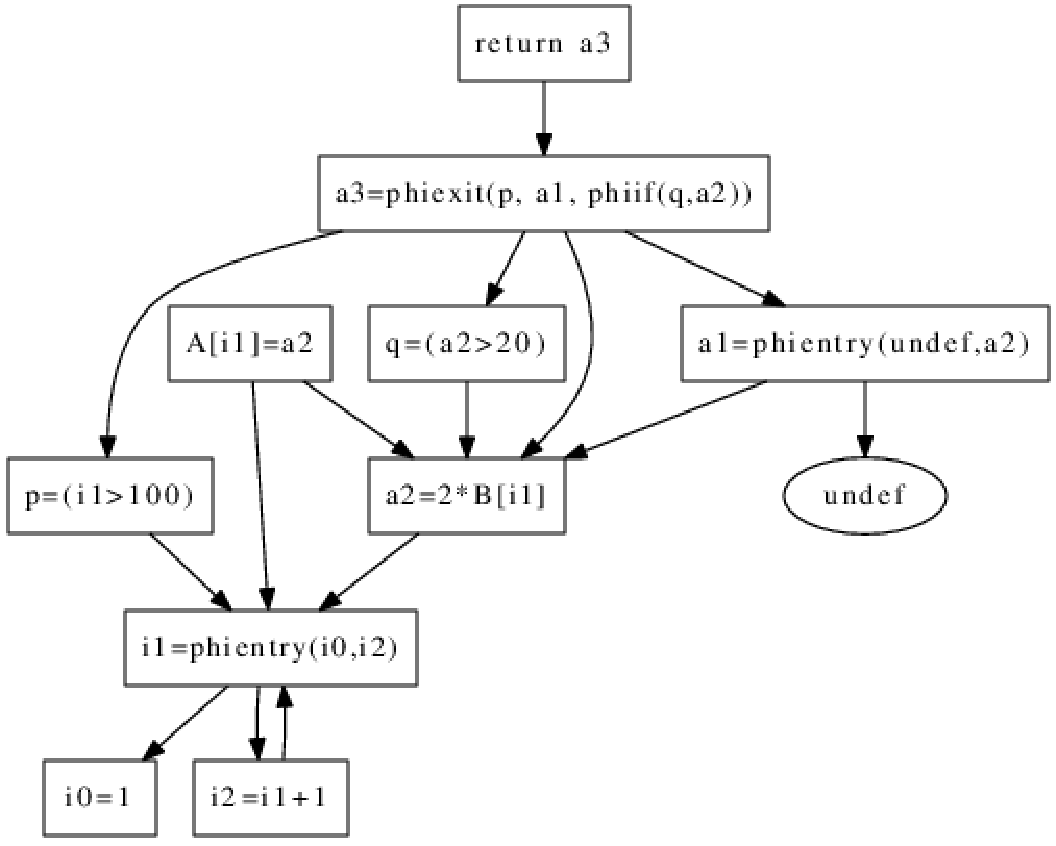
\includegraphics[scale=0.4]{gsa-example-2.pdf}
   \useheightbox{}
}
\caption{A graph representation of our sample code in (demand-based) GSA form.}
\label{fig:gsa-graph-example}
\end{figure}

It is easiest to understand these gating functions by means of an example. 
Figure~\ref{fig:gsa-graph-example} shows how our earlier code in Figure~\ref{fig:pdg} translates into GSA form. 
Here, we can see the use of both $\phientry$ and $\phiexit$ gating functions. 
At the header of our sample loop, the \phifun has been replaced by a $\phientry$ function which determine between the initial and iterative value of $i$. 
After the loop has finished executing, the nested $\phiexit$ function selects the correct live-out version of $a$.

This example shows several interesting points. 
First, the semantic of both the $\phiexit$ and $\phiif$ are strict in their gate: 
here $a_1$ or $\phiexit(q,a_2)$ are not evaluated before $p$ is known~\footnote{As opposed to the $\psi$-function described in Chapter~\ref{chapter:psi_ssa} that would use syntax such as $a_3=\phi((p\wedge \lnot q)?a_1, (\lnot p\wedge q)?a_2)$ instead.}. 
Similarly, a $\phiif$ function that results from the nested if-then-else code of Figure~\ref{fig:vsdg:structured} would be itself nested as $a=\phiif(p,\phiif(q,a_2,a_3),a_1)$. 
Second, this representation of the program does not allow for an interpreter to decide whether an instruction with a side effect (such as $A[i_1]=a_2$ in our running example) has to be executed or not. 
Finally, computing the values of gates is highly related to the simplification of path expressions: 
in our running example $a_2$ should be selected when the path $\lnot p$ followed by $q$ (denoted $\lnot p . 
q$) is taken while $a_1$ should be selected when the path $p$ is taken; 
for our nested if-then-else example, $a_1$ should be selected either when the path $\lnot p . 
r$ is taken or when the path $\lnot p . 
\lnot r$ is taken which simplifies to $\lnot p$. 
Diverse approaches can be used to generate the correct nested $\phiif$ or $\phiexit$ gating functions.

\begin{figure}
\subfloat[structured code]{
  \begin{minipage}{0.25\linewidth}
  \defuseheight{
    \begin{algorithm}[H]
      $a_1\gets\dots$\;
      \eIf{$p$}{
        \eIf{$q$}{
          $a_2\gets\dots$\;
        }{
          $a_3\gets\dots$\;
        }}{
          \eIf{$r$}{
            \dots
          }{\dots
          }
      }
    \end{algorithm}
  }
  \end{minipage}
}
\kern-3em
\subfloat[PDG]{
  \begin{minipage}{.38\linewidth}
    % \tikzfigure{pdg-structured-a}
    % \fbox{\vbox to \ht\tempflbox{\vfil\hbox{\tikzfigure{pdg-structured-a}}\vfil}}
    \centerheight{\tikzfigure{pdg-structured-a}}
  \end{minipage}
}
\subfloat[$a=\phiif(p,\phiif(q,a_2,a_3),a_1)$]{
  \begin{minipage}{.38\linewidth}
    \centerheight{\tikzfigure{pdg-structured-b}}
  \end{minipage}
}
\caption{(a) A structured code; (b) the PDG (with region nodes ommited); (c) the DAG representation of the nested gated $\phiif$ \label{fig:vsdg:structured}}
\end{figure}

The most natural way uses a data-flow analysis that computes, for each program points and each variable, its unique reaching definition and the associated set of reaching paths. 
This set of paths is abstracted using a \emph{path expression}. 
If the code is not already under SSA, and if at a merge point of the CFG its predecessor basic blocks are reached by different variables, a \phifun is inserted. 
The gates of each operand is set to the path expression of its corresponding incoming edge. 
If a unique variable reaches all the predecessor basic blocks, the corresponding path expressions are merged. 
Of course, a classical path compression technique can be used to minimize the number of visited edges. 
One can observe the similarities with the \phifun placement algorithm described in Section~\ref{section:alternative_ssa_construction_algorithms:loop}.

There also exists a relationship between the control dependencies and the gates: 
from a code already under strict and conventional SSA form, one can derive the gates of a $\phiif$ function from the control dependencies of its operands. 
This relationship is illustrated by Figure~\ref{fig:vsdg:structured} in the simple case of a structured code.
 
These gating functions are important as the concept will form components of the Value State Dependence Graph later. 
GSA has seen a number of uses in the literature including analysis and transformations based on data flow. 
With the diversity of applications (see chapters~\ref{chapter:hardware_compilation} and~\ref{chapter:loop_tree}), many variants of GSA have been proposed. 
Those variations concern the correct handling of loops in addition to the computation and representation of gates.


By using gating functions it becomes possible to construct IRs based solely on data dependencies. 
These IRs are sparse in nature compared to the CFG, making them good for analysis and transformation. 
This is also a more attractive proposition than generating and maintaining both a CFG and DFG, which can be complex and prone to human error. 
One approach has been to combine both of these into one representation, as is done in the PDG. 
Alternatively, we can utilize gating functions along with a data-flow graph for an effective way of representing whole program information using data-flow information.

\subsection{Backwards symbolic analysis with GSA}
GSA is useful for performing symbolic analysis\index{analysis, symbolic}. 
Traditionally, symbolic analysis is performed by forward propagation of expressions through a program. 
However, complete forward substitution is expensive and can result in a large quantity of unused information and complicated expressions. 
Instead, \textit{backward}, demand-driven\index{analysis, demand-driven} substitutions can be performed using GSA which only substitutes \textit{needed} information. 
Consider the following program:

{
  \def\Expr{\textit{EXPR}}
  \def\JMAX{\textit{JMAX}}
  \newcommand\assert[1]{\textbf{assert}\left(#1\right)}
  
\begin{algorithm}[H]
  $\JMAX\gets\Expr$\;
  \eIf{$p$}{
    $J\gets\JMAX-1$\;
  }{
    $J\gets\JMAX$\;
  }
  $\assert{J\leq \JMAX}$\;
\label{fig:tupaduaexample}
\end{algorithm}

If forward substitutions were to be used in order to determine whether the assertion is correct, then the symbolic value of $J$ must be discovered, starting at the top of the program in statement at line~1. 
Forward propagation through this program results in statement at line~6 being
$$\assert{\textbf{if } p \textbf{ then } \Expr-1 \textbf{ else }\Expr)\leq \Expr}$$
thus the $\assert{}$ statement evaluates to \true. 
In real, non-trivial programs, these expressions can get unnecessarily long and complicated.


Using GSA instead allows for backwards, demand-driven substitutions. The program above has the following GSA form:

\begin{algorithm}[H]
  $\JMAX_1\gets\Expr$\;
  \eIf{$p$}{
    $J_1\gets\JMAX_1-1$\;
  }{
    $J_2\gets\JMAX_1$\;
  }
  $J_3\gets\phiif(p,J_1,J_2)$\;
  $\assert{J_3\leq \JMAX_1}$\;
\label{fig:tupaduagsasubs}
%\caption{Figure~\ref{fig:tupaduaexample} in GSA form.}
\end{algorithm}

Using this backwards substitution technique, we start at statement on line~7, and follow the SSA links of the variables from $J_3$. 
This allows for skipping of any intermediate statements that do not affect variables in this statement. 
Thus the substitution steps are:

    \begin{tabbing}
        ${J_3}$ \= = $\phiif(p,J_1,J_2$)\\
        \> = $\phiif(p,\JMAX_1 - 1,\JMAX_1)$
    \end{tabbing}

The backwards substitution then stops because enough information has been found, avoiding the redundant substitution of $\JMAX_1$ by $\Expr$. 
In non-trivial programs this can greatly reduce the number of redundant substitutions, making symbolic analysis significantly cheaper.

\section{Value state dependence graph}
The\index{value state dependence graph}\index{VSDG} gating functions defined in the previous section were used in the development of a sparse data-flow graph IR called the Value State Dependence Graph (VSDG). 
The VSDG is a directed graph consisting of operation nodes, loop and merge nodes together with value and state dependency edges. 
Cycles are permitted but must satisfy various restrictions. 
A VSDG represents a single procedure: 
this matches the classical CFG.
%
An example VSDG is shown in Figure~\ref{fig:fac}. 

\begin{figure}[!htb]
  \defineheight{\tikzfigure{example-fac}}

  \centering
  \subfloat[code]{\label{fig:fac-code}
    \centerheight{
      \begin{minipage}{2.2in}
      \begin{algorithm}[H]
        \Func{fac ($n$)}{
          \eIf{$n=1$}{
            $\textit{result}\gets n$\;
          }{
            $\textit{result}\gets \textit{fac}(n-1)$\;
          }
          \textbf{return } \textit{result}\;
        }
      \end{algorithm}
      \end{minipage}
  %% \begin{minipage}{2.2in}
  %%     \texttt{\begin{tabbing}
  %%         int \=fac(int n) \{\\
  %%           \> int result;\\
  %%           \> if(\=n == 1)\\
  %%           \> \> result = n;\\
  %%           \> else\\
  %%           \> \> result = n * fac(n - 1);\\
  %%           \> return result;\\
  %%         \}
  %%     \end{tabbing}}
  %% \end{minipage}
    }
  }
  \subfloat[VSDG]{\label{fig:fac-vsdg}
    \begin{minipage}[b]{.6\linewidth}
    \useheightbox{}
  \end{minipage}
}
\caption{A recursive factorial function, whose VSDG illustrates the key graph components---value dependency edges (solid lines), state dependency edges (dashed lines), a \instruction{const} node, a \instruction{call} node, a \Gn, a conditional node, and the function entry and exit nodes.}
\label{fig:fac}
\end{figure}

%%%%%%%%%%%%%%%%%%%%%%%%%%%%%%%%%%%%%%%%%%%%%%%%%%%%%%%%%%%%%%%%%%%%%%%%%%%%%%%%

\subsection{Definition of the VSDG}

A VSDG is a labeled directed graph $G=(N,E_V,E_S,\ell,N_0,N_\infty)$ consisting of nodes $N$ (with unique entry node $N_0$ and exit node $N_\infty$), value dependency edges $E_V \subseteq N \times N$, state dependency edges $E_S \subseteq N \times N$. 
The labelling function $\ell$ associates each node with an operator.

The VSDG corresponds to a reducible program, e.g.~there are no cycles in the VSDG except those mediated by \Tns (loop).

Value dependency ($E_V$) indicates the flow of values between nodes. 
State dependency ($E_S$) represents two things; 
the first is essentially a sequential dependency required by the original program, e.g.~a given \texttt{load} instruction may be required to follow a given \texttt{store} instruction without being re-ordered, and a \texttt{return} node in general must wait for an earlier loop to terminate even though there might be no value-dependency between the loop and the \texttt{return} node. 
The second purpose is that state dependency edges can be added incrementally until the VSDG corresponds to a unique CFG. 
Such state dependency edges are called {\em serializing} edges\index{VSDG, serializing edge}.

The VSDG is implicitly represented in SSA form: 
a given operator node, $n$, will have zero or more $E_V$-consumers using its value. 
Note that, in implementation terms, a single register can hold the produced value for consumption at all consumers; 
it is therefore useful to talk about the idea of an output {\em port} for $n$ being allocated a specific register, $r$, to abbreviate the idea of $r$ being used for each edge $(n_1,n_2)$ where $n_2 \in \textit{succ}(n_1)$.
%Similarly, we will talk about (say) the
%``right-hand input port'' of a subtraction instruction, or of the $R$-input of
%a \Tn.

%%%%%%%%%%%%%%%%%%%%%%%%%%%%%%%%%%%%%%%%%%%%%%%%%%%%%%%%%%%%%%%%%%%%%%%%%%%%%%%%
%%
%%		NODE PROPERTIES
%%
%%%%%%%%%%%%%%%%%%%%%%%%%%%%%%%%%%%%%%%%%%%%%%%%%%%%%%%%%%%%%%%%%%%%%%%%%%%%%%%%

There are four main classes of VSDG nodes: 
value nodes (representing pure arithmetic)\index{VSDG, value nodes}, \Gns\ (conditionals)\index{VSDG, \Gns}, \Tns\ (loops)\index{VSDG, \Tns}, and state nodes\index{VSDG, state nodes} (side effects). 
The majority of nodes in a VSDG generate a value based on some computation (add, subtract, etc.) applied to their dependent values (constant nodes, which have no dependent nodes, are a special case).


%%%%%%%%%%%%%%%%%%%%%%%%%%%%%%%%%%%%%%%%%%%%%%%%%%%%%%%%%%%%%%%%%%%%%%%%%%%%%%%

\paragraph{\Gns}
The\index{VSDG, \Gns} \Gn\ is similar to the $\phiif$ gating function in being dependent on a control predicate, rather than the control-independent nature of SSA \phifuns.
A \Gn\ $\gamma(C:p,\ T:v_{\true},\ F:v_{\false})$ evaluates the condition dependency $p$, and returns the value of $v_{\true}$ if $p$ is true, otherwise $v_{\false}$.
We generally treat \Gns\ as single-valued nodes (contrast \Tns, which are treated as tuples), with the effect that two separate \Gns\ with the same condition can be later combined into a tuple using a single test. 
Figure~\ref{fig:twinPhis} illustrates two \Gns\ that can be combined in this way. 
Here, we use a pair of values (2-tuple) of values for prots $T$ and $F$. 
We also see how two syntactically different programs can map to the same structure in the VSDG.

\begin{figure}[!hb]
\subfloat[two different code schemes]{
  \begin{minipage}[c]{.35\linewidth}
  \defuseheight{
    \vbox{
    \begin{algorithm}[H]
      \eIf{p}{
        $x\gets 2$\;
        $y\gets 3$\;
      }{
        $x\gets 4$\;
        $y\gets 5$\;
      }
    \end{algorithm}
    \begin{algorithm}[H]
      \eIf{p}{
        $x\gets 2$\;
      }{
        $x\gets 4$\;
      }
      \eIf{p}{
        $y\gets 3$\;
      }{
        $y\gets 5$\;
      }
    \end{algorithm}
    }
  }
  \end{minipage}
}
\hfill
\subfloat[same \Gn]{
  \begin{minipage}[c]{.5\linewidth}
    \centerheight{\tikzfigure{vsdg-gammanodes}}
  \end{minipage}
}
\caption{Two different code schemes map to the same \Gn\ structure.}

\label{fig:twinPhis}
\end{figure}

%%%%%%%%%%%%%%%%%%%%%%%%%%%%%%%%%%%%%%%%%%%%%%%%%%%%%%%%%%%%%%%%%%%%%%%%%%%%%%%%

\paragraph{\Tns}
The\index{VSDG, \Tns} \Tn\ models the iterative behavior of loops, modeling loop state with the notion of an \emph{internal value} which may be updated on each iteration of the loop. 
It has five specific elements which represent dependencies at various stages of computation. 
The \Tn\ corresponds to a merge of the $\phientry$ and $\phiexit$ nodes in Gated SSA.
%
A \Tn\ $\theta(C:p,\ I:v_\textit{init},\ R:v_\textit{return},\ L: v_\textit{iter},\ X:v_{exit})$ sets its internal value to initial value $v_\textit{init}$ then, while condition value $p$ holds \true, sets $v_\textit{iter}$ to the current internal value and updates the internal value with the repeat value $v_\textit{return}$. 
When $p$ evaluates to \false computation ceases and the last internal value is returned through $v_\textit{exit}$.

%
A loop which updates $k$ variables will have: 
a single condition $p$, initial values $v_{\textit{init}}^1,\ldots,v_{\textit{init}}^k$, loop iterations $v_{\textit{iter}}^1,\ldots,v_{\textit{iter}}^k$, loop returns $v_{\textit{return}^1},\ldots,v_{\textit{return}}^k$, and loop exits $v_{\textit{exit}}^1,\ldots,v_{\textit{exit}}^k$.
The example in Figure~\ref{fig:thetatuple} also shows a pair (2-tuple) of values being used on ports $I,R,L,X$, one for each loop-variant value.

\begin{figure}[!ht]
  \defineheight{\tikzfigure{vsdg-theta}}
  \centering
  \subfloat[code]{
    \centerheight{
      \begin{minipage}[b]{0.20\linewidth}
      \begin{algorithm}[H]
        $j\gets \dots$\;
        $i\gets 0$\;
        \While{$i<10$}{
          $j\gets j-1$\;
          $i\gets i+1$\;
        }
        $\dots \gets j$
      \end{algorithm}
    \end{minipage}}
  }
%% \begin{verbatim}
%% j = ...
%% for(i = 0; 
%%     i < 10; 
%%     ++i)
%%          --j;	 
%% ... = j;
  %% \end{verbatim}
  \hfill
  \subfloat[VSDG]{
    \begin{minipage}[b]{.63\linewidth}
      \useheightbox{}
    \end{minipage}
  %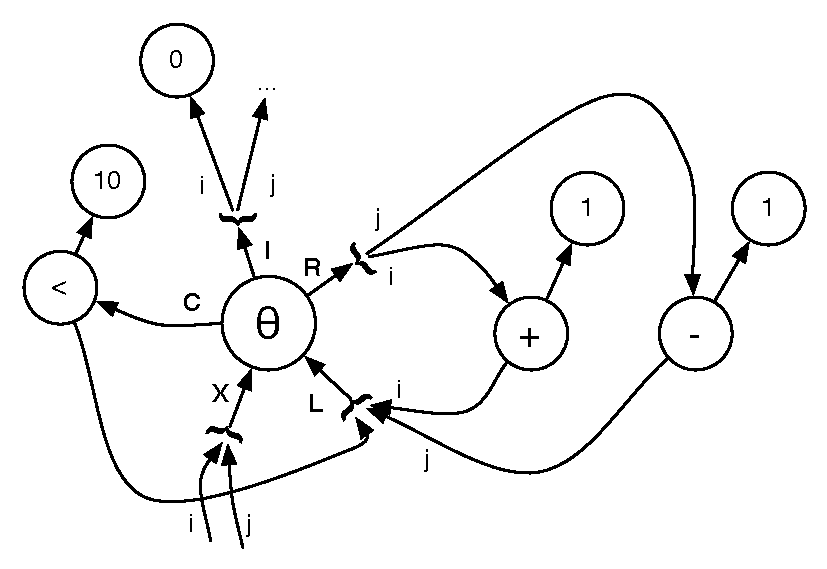
\includegraphics[scale=0.6]{vsdg-theta}
  }

\caption{An example showing a \texttt{for} loop. 
  Evaluating \textbf{X} triggers it to evaluate the \textbf{I} value (outputting the value \textbf{L}). 
  While \textbf{C} evaluates to true, it evaluates the \textbf{R} value (which in this case also uses the $\theta$-node's \textbf{L} value). 
  When \textbf{C} is false, it returns the final internal value through \textbf{X}. 
  As \texttt{i} is not used after the loop there is is no dependency on \texttt{i} at \textbf{X}.}
\label{fig:thetatuple}
\end{figure}

The \Tn\ directly implements pretest loops (\instruction{while}, \instruction{for}); 
post-test loops (\instruction{do...while}, \instruction{repeat...until}) are synthesized from a pre-test loop preceded by a duplicate of the loop body. 
At first this may seem to cause unnecessary duplication of code, but it has two important benefits: 
(1)~it exposes the first loop body iteration to optimization in post-test loops (cf.~loop-peeling), and (2)~it normalizes all loops to one loop structure, which both reduces the cost of optimization, and increases the likelihood of two schematically dissimilar loops being isomorphic in the VSDG.

%%%%%%%%%%%%%%%%%%%%%%%%%%%%%%%%%%%%%%%%%%%%%%%%%%%%%%%%%%%%%%%%%%%%%%%%%%%%%%%%

\paragraph{State nodes}
Loads and stores compute a value and state\index{VSDG, state nodes}. 
The \instruction{call} node takes both the name of the function to call and a list of arguments, and returns a list of results; 
it is treated as a state node as the function body may read or update state.

\medskip

We maintain the simplicity of the VSDG by imposing the restriction that \emph{all} functions have \emph{one} return node (the exit node $N_\infty$), which returns at least one result (which will be a state value in the case of \instruction{void} functions). 
To ensure that function calls and definitions are able to be allocated registers easily, we suppose that the number of arguments to, and results from, a function is smaller than the number of physical registers---further arguments can be passed via a stack as usual.

Note also that the VSDG neither forces loop invariant code into nor out-of loop bodies, but rather allows later phases to determine, by adding serializing edges, such placement of loop invariant nodes for later phases.

\subsection{Dead node elimination with the VSDG}
By representing a program as a VSDG, many optimizations become trivial. 
For example, consider dead node elimination\index{dead node elimination} (Figure~\ref{fig:dnevsdg}). 
This combines both dead code elimination\index{dead code elimination} and unreachable code elimination. 
Dead code generates VSDG nodes for which there is no value or state dependency path from the \texttt{return} node, i.e., the result of the function does not in any way depend on the results of the dead nodes. 
Unreachable code generates VSDG nodes that are either dead, or become dead after some other optimization. 
Thus, a \textit{dead node} is a node that is not post dominated by the exit node $N_{\infty}$. 
To perform dead node elimination, only two passes are required over the VSDG resulting in linear runtime complexity: 
one pass to identify all of the live nodes, and a second pass to delete the unmarked (i.e., dead) nodes. 
It is safe because all nodes which are deleted are guaranteed never to be reachable from the \texttt{return} node.

\begin{algorithm}[!ht]
{\bf Input:} A VSDG $G(N,E_V,E_S,N_{\infty})$ with zero or more dead nodes\;
{\bf Output:} A VSDG with no dead nodes\;
$\textit{WalkAndMark}(N_{\infty},G)$\;
$\textit{DeleteMarked}(G)$\;
\vspace{1em}
\Func{WalkAndMark($n,G$)}{
  \lIf{$n$ is marked}{\textbf{return}}
  mark $n$\;
  \ForEach{node $m \in N \wedge (n,m) \in (E_V \cup E_S)$}{
    $\textit{WalkAndMark}(m)$\;
  }
}
\vspace{1em}
\Func{DeleteMarked($G$)}{
  \ForEach{node $n \in N$}{
    \lIf{$n$ is unmarked}{$\textit{delete}(n)$}\;
  }
}
\caption{Dead node elimination on the VSDG.}
\label{fig:dnevsdg}
\end{algorithm}

\section{Further readings}
A compiler's intermediate representation can be a graph, and many different graphs exist in the literature. 
We can represent the control flow of a program as a Control-Flow Graph (CFG)~\cite{Alle70}, where straight-line instructions are contained within basic blocks and edges show where the flow of control may be transferred to once leaving that block. 
A CFG is traditionally used to convert a program to SSA form~\cite{Cytron:1991:TOPLAS}. 
We can also represent programs as a type of Data-flow Graph (DFG)~\cite{dennis74first,dennis80data}, and SSA can be represented in this way as an SSA Graph~\cite{504710}. 
An example was given that used the SSA Graph to detect a variety of induction variables\index{scalar evolution} in loops~\cite{Wolfe92,Ger95}. 
It has also been used for performing instruction selection\index{code selection} techniques~\cite{1375663,1269857}, operator strength reduction\index{strenght reduction}~\cite{504710}, rematerialization\index{rematerialization}~\cite{rematerialization}, and has been combined with an extended SSA language to aid compilation in a parallelizing\index{parallelisation} compiler~\cite{Stoltzextendedssa}.

% cite Harrold.
The Program Dependence Graph (PDG)\index{program dependence graph} as defined by Ferrante et al.~\cite{ferrantePDG} represents control and data dependencies in one graph. 
%Their definition of control dependencies that turns out to be equivalent to the post-dominance frontier leads to confusions at it uses a non-standard definition of post-dominance. 
We choose to report the definition of Bilardi and Pingali~\cite{Bilardi1996}. 
Section~\ref{section:vsdg:pdg} mentions possible abstractions to represent data dependencies for dynamically allocated objects. 
Among others, the book of Darte et al.~\cite{DarteRV-book} provides a good overview of such representations. 
The PDG has been used for program slicing\index{program slicing}~\cite{ottenstein84program}, testing~\cite{bates93incremental}, and widely for parallelization~\cite{ferrante85on,ferrante88generating,simons90a,baxter89program}. 
%We showed an example of how the PDG directly exposes parallel code.

Gating functions can be used to create directly interpretable \phifuns. 
These are used in Gated Single Assignment Form\index{gated single assignment}. 
Alpern et al.~\cite{AlpernWZ88} presented a precursor of GSA for structured code, to detect equality of variables. 
This chapter adopts their notations, i.e., a $\phiif$ for a if-then-else construction, a $\phientry$ for the entry of a loop, and a $\phiexit$ for its exit. 
The original usage of GSA was by Ballance et al.~\cite{ottenstein90program} as an intermediate stage in the construction of the Program Dependence Web IR. 
Further GSA papers replaced $\phiif$ by $\gamma$, $\phientry$ by $\mu$, and ~$\phiexit$ by $\eta$. 
Havlak~\cite{Havlak93constructionof} presented an algorithm for construction of a simpler version of GSA---Thinned GSA---which is constructed from a CFG in SSA form. 
The construction technique sketched in this chapter is developed in more detail in~\cite{207115}. 
GSA has been used for a number of analyses and transformations based on data flow. 
The example given of how to perform backwards demand-driven symbolic analysis using GSA has been borrowed from~\cite{Tu95gated}. 
If conversion (see Chapter~\ref{chapter:if_conversion}), converts control dependencies into data dependencies. 
To avoid the potential loss of information related to the lowering of \phifuns into conditional moves or select instructions, gating $\psi$-functions (see Chapter~\ref{chapter:psi_ssa}) can be used.

We then described the Value State Dependence Graph (VSDG)~\cite{UCAM-CL-TR-607}, which is an improvement on a previous, unmentioned graph, the Value Dependence Graph~\cite{177907}. 
It uses the concept of gating functions, data dependencies and state to model a program. 
We gave an example of how to perform dead node elimination on the VSDG. 
Detailed semantics of the VSDG are available~\cite{UCAM-CL-TR-607}, as well as semantics of a related IR: 
the Gated Data Dependence Graph~\cite{upton}. 
Further study has taken place on the problem of generating code from the VSDG~\cite{DBLP:conf/pdpta/Upton03,UCAM-CL-TR-705,stanier11thesis}, and it has also been used to perform a combined register allocation and code motion algorithm~\cite{Johnsoncombinedcode}.
